\documentclass[12pt,a4paper]{article}
\usepackage[UTF8]{ctex}
\usepackage{amsmath,amssymb}
\usepackage{xcolor}
\usepackage{hyperref}
\usepackage{geometry}
\usepackage{graphicx}
\geometry{margin=2.5cm}

\title{Hamiltonian Simulation / 哈密顿量模拟}
\author{QuoNic}
\date{}

\begin{document}
\maketitle

\begin{center}
\textbf{Simulation / 模拟} | 难度：高级 | 预计时间：20 分钟
\end{center}

\tableofcontents
\newpage

\section{为什么需要？}

哈密顿量模拟用于模拟量子系统的演化。

\subsection{经典局限}
\begin{itemize}
  \item 经典模拟需要指数时间
  \item 对于大系统，经典方法效率低
\end{itemize}

\subsection{量子优势}
\begin{itemize}
  \item 量子模拟可以在多项式时间内完成
  \item 提供指数加速
  \item 是量子化学的基础
\end{itemize}

\subsection{实际应用}
\begin{itemize}
  \item 量子化学
  \item 材料科学
  \item 量子物理
\end{itemize}

\section{快速上手}

\begin{verbatim}
from quonic.simulation import hamiltonian_simulation
result = hamiltonian_simulation(H=[[1,0],[0,-1]], t=1.0)
print(f'Evolution: {result.evolution}')
\end{verbatim}

\textbf{预期输出}：
\begin{verbatim}
Evolution: [[0.54+0.84j, 0], [0, 0.54-0.84j]]
\end{verbatim}

\section{原理详解}

\subsection{电路图}

\begin{center}
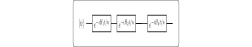
\includegraphics[width=0.6\textwidth]{../../images/hamiltonian_simulation_circuit.svg}
\end{center}

\subsection{数学推导}

哈密顿量模拟：
\begin{equation}
U(t) = e^{-iHt}
\end{equation}

\textbf{Trotter 分解}：
\begin{equation}
e^{-iHt} \approx \prod_k e^{-iH_k \Delta t}
\end{equation}

\subsection{几何解释}

哈密顿量模拟在量子态空间中演化。

\section{代码详解}

\begin{verbatim}
from quonic.simulation import hamiltonian_simulation

# hamiltonian_simulation(H, t)
# H: Hamiltonian matrix
# t: evolution time
result = hamiltonian_simulation(H=[[1,0],[0,-1]], t=1.0)
print(f'Evolution: {result.evolution}')
\end{verbatim}

\section{进阶用法}

\subsection{场景 1：不同哈密顿量}

\begin{verbatim}
from quonic.simulation import hamiltonian_simulation
result = hamiltonian_simulation(H=[[0,1],[1,0]], t=1.0)
print(f'Evolution: {result.evolution}')
\end{verbatim}

\section{适用场景}

\subsection{量子化学}

哈密顿量模拟可以用于模拟分子系统。

\subsection{材料科学}

哈密顿量模拟可以用于设计新材料。

\section{常见问题}

\subsection{哈密顿量模拟和动力学模拟有什么区别？}

哈密顿量模拟关注演化算子，动力学模拟关注态演化。

\subsection{哈密顿量模拟的精度如何？}

取决于 Trotter 分解的阶数。

\section{学习路径}

\subsection{前置知识}
\begin{itemize}
  \item Trotter 分解
  \item 量子相位估计
  \item 量子傅里叶变换
\end{itemize}

\subsection{继续学习}
\begin{itemize}
  \item 量子化学
  \item 材料科学
  \item 量子物理
\end{itemize}

\section{完整示例代码}

\subsection{示例 1：基本哈密顿量模拟}

\begin{verbatim}
from quonic.simulation import hamiltonian_simulation
result = hamiltonian_simulation(H=[[1,0],[0,-1]], t=1.0)
print(f'Evolution: {result.evolution}')
\end{verbatim}

\section{下载}

\begin{itemize}
  \item [hamiltonian\_simulation.py](https://github.com/ChrisLee0721/QuoNic/blob/main/examples/hamiltonian_simulation/hamiltonian_simulation.py)
\end{itemize}

\end{document}
